\section{Environment map}
\label{sec:chapter_stato_arte_envmap}

Nella grafica computazionale, una environment map è un’efficiente tecnica utilizzata per approssimare la riflessione e rifrazione di oggetti tramite l’utilizzo di una texture precomputata.
La texture rappresenta l’ immagine dell’ ambiente che circonda uno o più oggetti nella scena.
L’ Environment map si basa principalmente su due assunzioni:
\begin{itemize}
\item L’ambiente è infinitamente distante dagli oggetti.
\item Gli oggetti non possono riflettere se stessi.
\end{itemize}
La prima assunzione permette di accedere alla environment map tramite la sola direzione in cui guarda l’osservatore. Il fatto che la env map non dipenda dalla sua posizione comporta però errori nella riflessione quando l’ambiente non è sufficientemente distante. 
\\
In tal caso è molto probabile che gli oggetti riflessi da un oggetto possano apparire in posizioni sbagliate.
\\
Questo errore è particolarmente riscontrabile su superfici in cui la riflessione dipende pesantemente dalla posizione (come gli specchi), mentre risulta quasi impercettibile su superfici curve. 
\\
Il presente aspetto verrà analizzato più nel dettaglio a fine paragrafo.
La seconda assunzione invece non permette di ottenere riflessioni multiple come ad esempio quelle ottenute da due oggetti vicini che si riflettono tra loro. Per questo motivo, è preferibile utilizzare l’environment map su oggetti convessi piuttosto che su oggetti concavi, i quali riflettono se stessi.
\\
Un oggetto viene detto convesso se comunque vengono presi due punti che gli appartengono anche il segmento che li congiunge gli appartiene interamente. In caso contrario l’ oggetto viene detto concavo. \cite{env1}
\begin{figure}[htb]
 \centering
 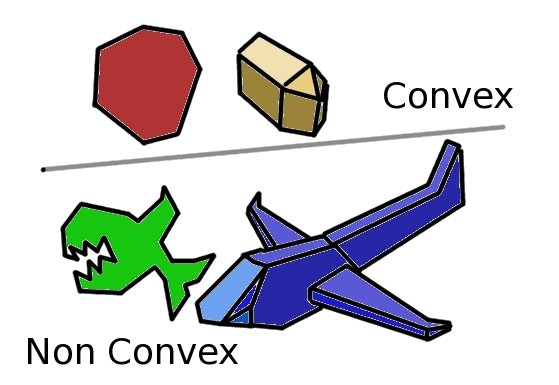
\includegraphics[width=0.5\linewidth]{images/chapter_stato_arte/stato_arte_conc_conv.jpg}\hfill
 \caption[Concavo,convesso]{Differenza tra oggetti convavi e convessi.}
 \label{fig:stato_arte_conc_conv}
\end{figure}
L’env map viene utilizzata ancora oggi nei videogiochi moderni permettendo di alleggerire notevolmente il carico computazionale del rendering real-time per la realizzazione di superfici riflettenti o rifrangenti.
\\
\begin{figure}[htb]
 \centering
 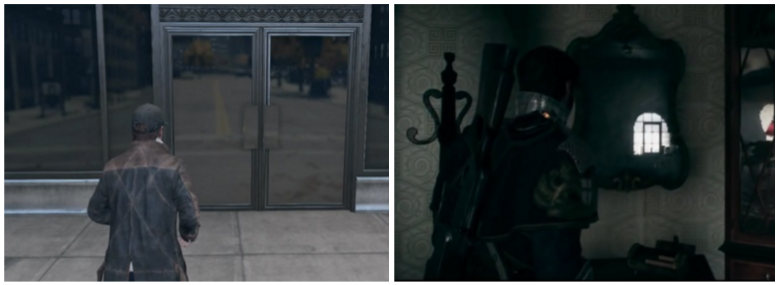
\includegraphics[width=1\linewidth]{images/chapter_stato_arte/stato_arte_wd_to.png}\hfill
 \caption[Le env map nei videogiochi]{Le env map sono tutt'oggi di ampio utilizzo in ambiente videoludico.}
 \label{fig:stato_arte_wd_to}
\end{figure}
\\
Videogiochi recenti quali Watch Dogs (a sinistra) e The Order: 1886 (a destra) ne fanno ampio utilizzo in quanto questa tecnica permette di ottenere un frame-rate costante anche in presenza di effetti complessi di riflessione e rifrazione. Siccome la texture utilizzata durante l’algoritmo di env-map è precomputata e rimane fissa, non è possibile però ottenere la riflessione/rifrazione dinamica di oggetti o personaggi in movimento (in entrambe le figure è possibile notare come  il personaggio in movimento non venga riflesso). Compromesso comunque accettabile in quanto il calcolo real-time di questi effetti potrebbe provocare una drastica diminuzione del frame-rate.
Nel presente lavoro di tesi l’utilizzo delle env-map ben si addiceva al contesto di lavoro preso in riferimento. Le scene di interni di appartamenti risultano infatti fisse nel tempo,  cosa che ha permesso di sfruttare questa tecnica per mantenere costanti le prestazioni dell’ applicazione anche in presenza di molti effetti di riflessione e rifrazione.

\subsection{L'algoritmo di environment-mapping}
\label{sec:chapter_stato_arte_algo_envmapping}

L’algoritmo di environment-mapping si comporta in maniera differente per superfici riflettenti e rifrangenti. Questo perchè le due superfici deviano in maniera differente i raggi che le colpiscono.
Le superfici riflettenti, riflettono il raggio di incidenza $i$ (partito dall’ occhio dell’ osservatore) che le colpisce in una direzione $r$ dipendente dalla normale $n$ sulla superficie.
\\
\begin{figure}[htb]
 \centering
 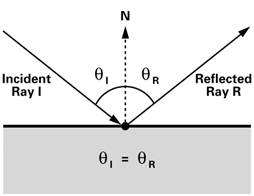
\includegraphics[width=0.5\linewidth]{images/chapter_stato_arte/stato_arte_inc_refl.png}\hfill
 \caption[Env map: riflessione]{Comportamento del raggio di incidenza i quando si ha un effetto di riflessione.}
 \label{fig:stato_arte_inc_refl}
\end{figure}

Per superfici perfettamente riflettenti (ad esempio uno specchio) l’angolo di incidenza $\Theta_i$ è lo stesso dell’ angolo di riflessione $\Theta_r$.
Il calcolo del vettore $r$ è essenziale per l’ algoritmo di env-map di riflessione ed il suo utilizzo verrà spiegato a breve durante la trattazione completa dei passi dell’algoritmo.
\begin{equation}
r = i - 2(n * i)n 
\end{equation}
Le superfici rifrangenti, invece, rifrangono  il raggio di incidenza $i$ che le colpisce in una direzione $t$ dipendente dal mezzo attraversato.
\\
\begin{figure}[htb]
 \centering
 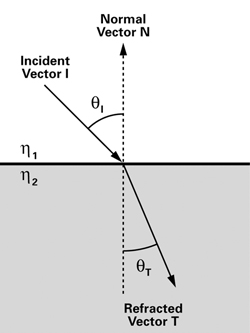
\includegraphics[width=0.4\linewidth]{images/chapter_stato_arte/stato_arte_refr.png}\hfill
 \caption[Env map: rifrazione]{Comportamento del raggio di incidenza i quando si ha un effetto di rifrazione.}
 \label{fig:stato_arte_refr}
\end{figure}
\\
La \emph{legge di Snell} \cite{env2} descrive la relazione tra l’ angolo di incidenza e di rifrazione di un raggio che transita tra due mezzi con indice di rifrazione differente.
\begin{equation}
n_1sin\Theta_1 = n_2sin\Theta_2 
\end{equation}
L’ equazione prevede quattro variabili: l’angolo di incidenza $\Theta_i$, l’angolo di rifrazione $\Theta_t$, l’indice di rifrazione del primo mezzo attraversato $n_1$ e l’indice di rifrazione del secondo mezzo attraversato $n_2$.
L’ indice di rifrazione è una grandezza adimensionale specifica per un mezzo che quantifica la diminuzione della velocità di propagazione della luce quando esso viene attraversato. Maggiore è l’indice di rifrazione per un mezzo, minore è la velocità di propagazione.
Nella figura l’indice di rifrazione $n_2$ è maggiore dell’ indice di rifrazione $n_1$. 
Siccome la velocità di propagazione è minore nel secondo mezzo rispetto al primo, anche l’angolo di rifrazione è minore rispetto all’angolo di incidenza (l’angolo è più vicino alla normale). 
L’equazione permette il calcolo del vettore $t$, essenziale per l’algoritmo di env-map di rifrazione:
\begin{equation}
t = \frac{\eta_1}{\eta_2}i + (\frac{\eta_1}{\eta_2}cos\Theta_i - \sqrt[2]{1 - sin^2\Theta_t})n
\end{equation}
Il calcolo del vettore $r$ e del vettore $t$ è semplice e questo rende l’environment map il metodo più veloce per renderizzare una superficie che rifrae o riflette.
L’ env-map prende il nome di \emph{env-map di riflessione} , quando viene utilizzata per simulare la riflessione e di \emph{env-map di rifrazione} quando viene utilizzata per simulare la rifrazione. Nulla vieta di utilizzare la stessa env-map per simulare entrambi gli effetti.
L’algoritmo usa il vettore $r$ quando viene utilizzata una env-map di riflessione e $t$ quando viene utilizzata una env-map di rifrazione.
Le operazione che l’ algoritmo effettua sono le seguenti: \cite{real_time_book}
\begin{itemize}
\item Generare o caricare una immagine a due dimensioni che rappresenta l’ ambiente ( l’env-map stessa).
\item Per ogni pixel che contiene un oggetto riflettente, calcolare la normale alla superficie dell’oggetto.
\item Computare il vettore $r$ oppure il vettore $t$.
\item Usare il vettore scelto come indice nella env-map per prelevare il valore che rappresenta la radianza entrante nella direzione di $r$ o $t$.
\item Usare il dato ottenuto dalla environment map come radianza. 
\end{itemize}
\begin{figure}[htb]
\centering
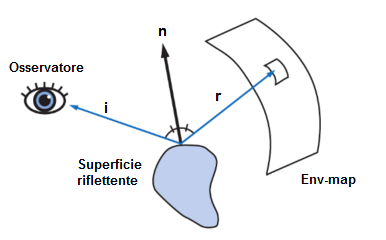
\includegraphics[width=0.6\linewidth]{images/chapter_stato_arte/stato_arte_env_alg.png}\hfill
\caption[Algoritmo environment mapping]{Environment mapping.}
\label{fig:stato_arte_env_alg}
\end{figure}
Il vettore r o t $(x,y,z)$, tramite una funzione di proiezione, viene convertito in un valore a due dimensioni $(u,v)$. Di fatto la env map viene utilizzata come una tabella a due dimensioni; il valore a due dimensioni viene utilizzato come indice e viene prelevato il valore di radianza del pixel da mostrare su schermo.
\\
Questo approccio produce risultati simili al ray tracing per quanto riguarda la riflessione o rifrazione, risultando però  più efficiente. 
Calcolare l’ angolo di incidenza e riflessione seguito da una ricerca nella env-map rispetto a calcolare l’esatta riflessione o rifrazione della luce tracciando un raggio e seguendo il suo percoso ottico semplifica di molto il lavoro eseguito dalla GPU. 

Esistono però problemi nell’ utilizzo della env map su superfici piatte in quanto i raggi che da esse vengono riflessi variano pochissimo in termini di angolazione. Questo si traduce in una proiezione delle componenti $(x,y,z)$ di $r$ o di $t$ in valori $(u,v)$ che sono molto simili per tutti i raggi riflessi dalla superficie. In questo modo i valori $(u,v)$ indicizzano solo una piccola porzione della tabella (env map) e questa porzione viene mappata su una superficie potenzialmente più larga. Il risultato visibile sulla superficie è quindi quello che solamente una piccola porzione della envmap viene riflessa sulla superficie e quest’ ultima può risultare ingrandita.
Inoltre nel caso di env map di rifrazione, l’algoritmo simula solo il primo raggio rifratto.
\\
\begin{figure}[htb]
\centering
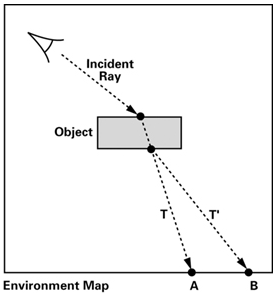
\includegraphics[width=0.5\linewidth]{images/chapter_stato_arte/stato_arte_refr_2.png}\hfill
\caption[Environment mapping: rifrazione]{Environment mappin: rifrazione}
\label{fig:stato_arte_refr_2}
\end{figure}
\newpage
Il raggio in realtà dovrebbe essere rifratto due volte: la prima quando entra nel mezzo, la seconda quando esce (vettore $T’$). Nella pratica però la seconda rifrazione non viene simulata ed il raggio prosegue nella direzione $T$ invece che in quella di $T’$. 
Questo tipo di semplificazione permette di alleggerire il carico di lavoro del render permettendo di ottenere una rifrazione convincente utilizzando un solo raggio.
Il risultato ottenuto da quest’ ultimo è sicuramente non accurato fisicamente come quello che si otterrebbe utilizzando due raggi ma comunque risulta molto simile.
Viene preferito questo approccio in quanto risulta più veloce e crea un credibile effetto di rifrazione.

\subsection{Env map cubica}
\label{sec:chapter_stato_arte_envmap_cubica}

Una env map cubica o cube map utilizza le immagini ottenute da sei facce di un cubo come env map \cite{env3} . 
L’ ambiente viene proiettato su ogni faccia del cubo e salvato tramite sei texture quadrate oppure disposte in sei diverse regioni di una singola texture (Fig. \ref{fig:stato_arte_cubo_envmap} ).
\begin{figure}[htb]
 \centering
 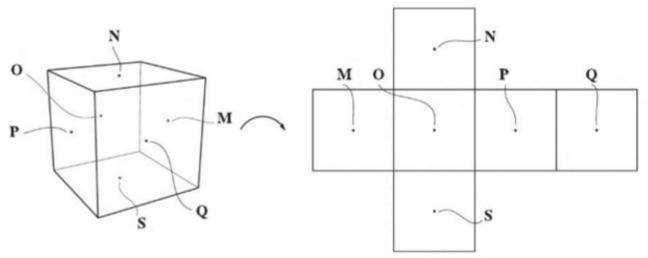
\includegraphics[width=0.6\linewidth]{images/chapter_stato_arte/stato_arte_cubo_envmap.png}\hfill
 \caption[Env map cubica]{Env map cubica}
 \label{fig:stato_arte_cubo_envmap}
\end{figure}
Nel dettaglio per ottenere una cube map, inizialmente viene piazzata una camera nella scena, successivamente viene proiettato l’ ambiente su ogni faccia di un cubo, disposto nel centro della camera, ed infine quest’ ultimo viene salvato su sei diverse texture quadrate o su una singola texture con sei diverse regioni cubiche (Fig. \ref{fig:stato_arte_texture_env_cubo} ).
\\
La scena viene quindi renderizzata sei volte (una per ogni faccia del cubo), con la camera posizionata al centro del cubo che guarda ad ogni faccia del cubo con un angolo di vista di 90 gradi.
\\
La forza di questo metodo è che l’ env map può essere facilmente generata real-time da qualsiasi renderer in quanto ha differenti vantaggi rispetto ad altre tecniche come le env-map sferica.
\\
L’ env map cubica, a differenza di quella sferica, è infatti indipendente dal punto di vista; infatti in applicazioni in cui il esso si muove non è necessario creare una nuova env-map per ogni nuovo punto di vista.
\begin{figure}[htb]
 \centering
 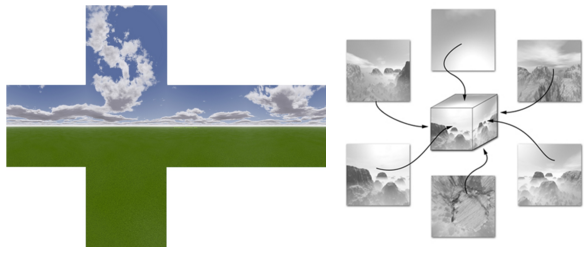
\includegraphics[width=0.9\linewidth]{images/chapter_stato_arte/stato_arte_texture_env_cubo.png}\hfill
 \caption[Env map texture]{Differenza tra una singola texture con sei regioni quadrate (sinistra), o sei texture quadrte distinte (destra).}
 \label{fig:stato_arte_texture_env_cubo}
\end{figure}